\RequirePackage[l2tabu, orthodox]{nag}%check for errors, obsoletion and warn helpfull
%-------------------
%Beginn des Kopfbereiches
%-------------------
\documentclass[a4paper,12pt,twoside]{scrreprt} 

%We speak german and english
\usepackage[utf8]{inputenc}
\usepackage[ngerman,english]{babel}

%Own style definitions:
\setkomafont{title}{\scshape}
\addtokomafont{disposition}{\itshape}
\setlength{\parindent}{2.4ex}
\setlength{\parskip}{0.7em}


%use garamond Font

\usepackage[T1]{fontenc}
\usepackage{textcomp}
\usepackage[urw-garamond]{mathdesign}
\usepackage{garamondx}
\renewcommand{\rmdefault}{ugm}

\clubpenalty10000
\widowpenalty10000
%\usepackage{microtype}%for tuned kerning
\usepackage{layouts}
%Math stuff
\usepackage{amsmath}
%\usepackage{pgfplots}
%Handy packages & Co
\usepackage{color}
\usepackage{blindtext}
\usepackage{setspace}
\usepackage{csquotes}
\usepackage{multicol}
\usepackage{units}
\usepackage{siunitx}
	\DeclareSIUnit\years{yrs}
\usepackage{physics}

\usepackage{placeins}
\usepackage[x11names]{xcolor}
%customize toc
\setcounter{tocdepth}{1}
\setcounter{secnumdepth}{2}
\numberwithin{equation}{chapter}


\usepackage[
    backend=biber,
    style=numeric,
    natbib=true,
    url=false, 
    doi=true,
    eprint=false
]{biblatex}
\usepackage[hidelinks,pdfusetitle]{hyperref}

\addbibresource{refs.bib}
%Own Commands

%Plot-texts
\newcommand{\DescrHeightLevels}{ For the vertical profile model levels have been used. For each level the mean height is used. Full model levels are taken to be in the geometric mean height between half levels. }

%\newcommand{\data}{./data}
\newcommand{\Ri}{R\!i}
\newcommand{\p}{\par}
\newcommand{\ftimes}{\cdot}
\newcommand{\ddiff}[2]{\ensuremath{\frac{d\! #1}{d\! #2}}}
\newcommand{\pdiff}[2]{\ensuremath{\frac{\partial\! #1}{\partial\! #2}}}
\newcommand{\euler}[1]{\ensuremath{\pdiff{#1}{t}+\left(\vec{v}\times\vec{\nabla}\right)#1}}



%Begin pgfplot stuff
\usepackage{pgfplots}
\pgfplotsset{compat=1.11}
\pgfplotstableset{col sep=semicolon}
\usepgfplotslibrary{units}
\def\axisdefaultheight{120pt}
\def\axisdefaultwidth{240pt}

\newcommand{\colA}{green}
\newcommand{\colB}{brown}
\newcommand{\colC}{blue}
\newcommand{\colD}{black}
\newcommand{\colE}{orange}


\pgfplotscreateplotcyclelist{fcolor}{%
Green4,mark=none\\%
Chocolate4\\%
RoyalBlue3\\%
black\\%
OrangeRed1\\%
}

\begin{document}
\chapter{Removing background tendencies}
\vspace{-0.6cm}
For a Variable $\Phi$ let $\Phi^R_0$ be the reanalysis field from which the model is started and $\Phi^R_1$ the next reanalysis field available after a time of $\Delta T$. For ensemble forecasts each member is always treated separately.
\p
 The forecast field for $t$ seconds after $\Phi^R_0$ is denoted $\Phi^M(t)$. The model time step numbered $0\leq i\leq n \in \mathbb{N}$ is $\Delta t$ seconds. Therefore model fields are available for $t=i\Delta t$ and called $\Phi^M_i$.
 \p
To find the true erroneous tendency we only want to consider the differences between the model tendency and the climatological background tendency, which can originate from diurnal or seasonal cycles. To achieve that we subtract the background tendency from the model tendency. The figure shows that the resulting difference between background and model tendency will equal the negative analyses increment.
\p
The Background tendency is $\dot{\Phi}^R=\nicefrac{(\Phi^R_1-\Phi^R_0)}{\Delta T}$ if $i<\nicefrac{\Delta T}{\Delta t}$, elsewise $\Phi^R_{2,3,\cdots}$ will be used such that the time step $i$ is in between the used reanalyses.
 The model tendency $\dot{\Phi}_i$ exclusive the background tendency between the time steps $i$ and $i+1$ is then calculated by:
\begin{equation}
\dot{\Phi}_i=\frac{\Phi^M_{i+1}-\Phi^M_i}{\Delta t}-\dot{\Phi}^R
\end{equation}
\p
Alternatively the model tendency (inclusive background tendencies) can also be computed as sum over k component tendencies: $\dot{\Phi}_i$:
\begin{equation}
\dot{\Phi}_i+\dot{\Phi}^R=\sum_k \dot{\varphi}^M_k
\end{equation}
\p
Here $\dot{\varphi}^M_k$ are the different model tendencies from the dynamics and physics of the NWP. It is important that all processes are included for this equation to hold.
\p
Time-mean tendencies between $\dot{\Phi}_i$ to $\dot{\Phi}_j$ are obtained by:
\begin{equation}
\dot{\Phi}_{ij}=\frac{1}{j-i}\sum_{k=i}^{j-1}\dot{\Phi}_k=\frac{\Phi^M_{j}-\Phi^M_i}{(j-i)\Delta t}-\dot{\Phi}^R\qqtext{with:} i<j\leq n
\end{equation}
\p
For $i=0\text{ and } j=n$ where $n$ denotes the cycling interval used in the data assimilation $\dot{\Phi}_{ij}$ will equal the negative analysis increment. (see figure)
\p
\FloatBarrier
\begin{figure}
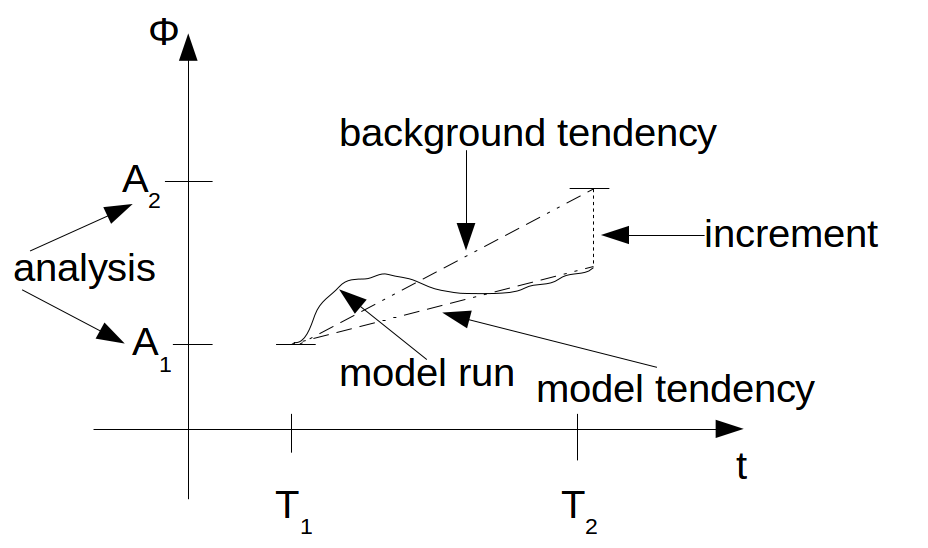
\includegraphics[scale=0.9]{./img/sketch2.png} 
\caption{Conceptual sketch of initial tendency method showing the background tendency $\dot{\Phi}^R$, model tendency $\dot{\Phi}_{0n}$, the analysis states $\Phi^R_{1/2}$ and the model run $\Phi^M(t)$}
\label{fig:1}
\end{figure}



\end{document}
